\documentclass[11pt]{article}

\def\dj{d\kern-0.4em\char"16\kern-0.1em}
\def\Dj{mbox{\raise0.3ex\hbox{-}\kern-0.4em D}}

\usepackage{geometry}
\usepackage{indentfirst}
\usepackage{multicol}
\usepackage{graphicx}

\geometry{
    left=10mm,
    right=60mm,
    top=20mm,
    bottom=20mm
}
\author{Ime i prezime}
\title{Eratosten}

\renewcommand{\contentsname}{Sadr\v zaj}

\setlength\parskip{1em}
\linespread{1.3}

\begin{document}

\maketitle
\thispagestyle{empty}
\newpage

\tableofcontents
\thispagestyle{empty}
\newpage

\pagestyle{plain}
%\pagenumbering{arabic}
\setcounter{page}{1}

\section{\v Zivot}

Ro\dj en je u Kireni\footnote{danas Shahhat, Libija}, a umro u ptolomejskoj Aleksandriji. Stekao je slavu kao prvi koji je upotrebio sistem \v sirina i du\v zina, te prvi koji je izra\v cunao Zemljinu veli\v cinu.


\bfseries
Eratosten se obrazovao u Aleksandriji i nekoliko godina u Atini. Ptolomej III Euergeta imenovao ga je 236. pne. predsednikom aleksandrijske biblioteke. Eratosten je dao nekoliko va\v znijih doprinosa nauci. Bio je dobar prijatelj s Arhimedom. Oko 255. pne. je izumeo armilarnu sferu, koja se na\v siroko koristila sve do pronalaska planetarijuma u 18. veku.

\itshape
Eratosten je poznat pod imenom Beta (slovo i broj 2) jer se navodno dokazao kao drugi u svetu u mnogim podru\v cjima. Bio je na glasu po svom bahatom karakteru. Oslepeo je 195. pne., vi\v se nije mogao \v citati i godinu dana kasnije izgladneo se na smrt.
\mdseries \upshape

Eratosten je bio:
\begin{itemize}
    \item matemati\v car
    \item astronom
    \item geograf
    \item pesnik
\end{itemize}

\def\figurename{slika}
\begin{figure}[h!]
	\centering
	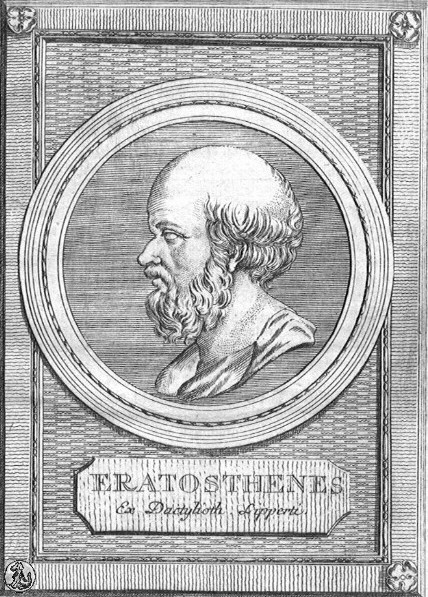
\includegraphics[width=0.5\textwidth]{Eratosthenes.jpg}
	\caption{Eratosten}
\end{figure}


\section{Pesni\v stvo}

\begin{multicols}{2}
U elegiji Erigoni pevao je ο ati\v ckom seljaku Ikariju, koji je prvi od Dionisa nau\v cio da sadi lozu, ali su ga pijani seljaci pogubili. Njegova \' cerka Erigona sa svojom vernom kujom nađe le\v s i obesi se i, naposletku, sve troje bude uvr\v steno me\dj u zvezde. Sli\v can sadr\v zaj ima sa\v cuvani prozni spis Pretvaranja u zvezde , u kojem izla\v zu pri\v ce ο postanku sazve\v z\dj a. Delo s tim nazivom, koje imamo i koje mu se pripisuje, nije njegovo. Od njegovih dela je vrlo malo sa\v cuvano. Fragmenti poezije pokazuju veliku ve\v stinu.

Dok je Eratosten kao pesnik hodao putem pesnika Kalimaha, prethodnika na \v celu Biblioteke, on ga je kao istra\v ziva\v c daleko prevazi\v sao. U svom velikom delu Ο staroj komediji on se bavio obiljem najrazli\v citijih pitanja i uticao na prou\v cavanja svojih naslednika Eufronija (u\v citelja Aristarhovog), Aristofana i Didima.
\end{multicols}

\section{Odre\dj ivanje obima Zemlje}

Oko 240. pne. Eratosten je izra\v cunao Zemljin opseg koriste\' ci se trigonometrijom i poznavanjem ugla Sun\v cevih zraka u odnosu na Zemlju u podne u Aleksandriji i Sieni (danas Asuan, Egipat). Ra\v cun je izveo pod pretpostavkom da je Zemlja okrugla i da je Sunce toliko udaljeno da se njegovi zraci mogu posmatrati kao paralelni.


\newpage
\begin{equation}
f(x) = \left\{
\begin{array}{rl}
\sqrt[3]{\sqrt{\frac{x}{6}}} \cdot \log_{e}{4 \pi} , & 0 \le x \le 6 \\
\lim\limits_{ n \rightarrow 6 } \frac{x^2n}{n} , & x > 6 \\
\sum\limits_{n=1}^{ +\infty} x^2 \cdot \frac{1}{n^2} , & inace
\end{array}
\right.
\end{equation}


\end{document} 